\documentclass[12pt, stu, floatsintext,table]{apa7}


\usepackage{booktabs}
\usepackage{float}
\usepackage{wrapfig}
\usepackage{subfig}
\usepackage{setspace}
\usepackage{caption}
\usepackage[section]{placeins}
\captionsetup[figure]{font=footnotesize,labelfont=small}

\makeatletter
\AtBeginDocument{%
  \expandafter\renewcommand\expandafter\subsection\expandafter
    {\expandafter\@fb@secFB\subsection}%
  \newcommand\@fb@secFB{\FloatBarrier
    \gdef\@fb@afterHHook{\@fb@topbarrier \gdef\@fb@afterHHook{}}}%
  \g@addto@macro\@afterheading{\@fb@afterHHook}%
  \gdef\@fb@afterHHook{}%
}
\makeatother

\title{EE 508 Final Project: An analysis of Franklin, MA CPA fund use for acquiring new open space}
\shorttitle{ }
\author{Rose Determan}
\affiliation{Boston University}
\course{EE 508: Data Science for Conservation Decisions}
\duedate{January 18, 2022}
\professor{ }
\begin{document}
\maketitle
\section{Introduction}
\begin{wrapfigure}{r}{0.5\textwidth}
  \begin{center}
    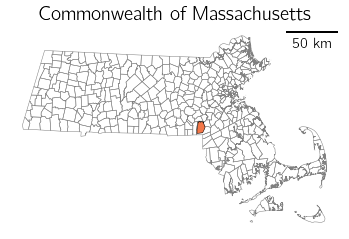
\includegraphics[width=0.48\textwidth]{figures/state.png}
  \end{center}
  \caption{Franklin, MA is highlighted in orange.}
\end{wrapfigure}

Franklin, MA is a municipality in the Commonwealth of Massachusetts 28 miles South of Boston, MA and 26 miles North of Providence, RI (Figure 1). As of the 2020 Annual Report, there was an estimated population of 33,644 individuals. 
On May 6, 2020 the town council approved the adoption of the Community Preservation Act (CPA) and town members voted in favor of the initiative on November 3, 2021. The Massachusetts Community Preservation Act, was originally signed into state law in 2000, and 187 cities and towns in Massachusetts have adopted the CPA. The goal of the CPA is to create a source of funds so communities can retain aspects of their town that fall outside of traditional municipal government jurisdictions. Municipalities contribute to their CPA fund from a surcharge on real property taxes, and the Commonwealth contributes to each municipality's fund (\emph{CPA: An Overview}) These funds can be used for
\begin{itemize}
  \setlength\itemsep{0.0em}
  \item the acquisition, creation and preservation of \textbf{open space}
  \item the acquisition, preservation, rehabilitation, and restoration of \textbf{historic resources}
  \item the acquisition, creation, preservation and rehabilitation and restoration of \textbf{land for recreational use}
  \item the acquisition, creation, preservation, rehabilitation and restoration, and support of \textbf{community housing} (Town of Franklin 2020 Annual Report)
\end{itemize}
Statewide, since 2000, 32,566 acres of open space have been preserved as part of CPA funded projects (\emph{CPA: An Overview}).    

\begin{wrapfigure}[18]{r}{0.5\textwidth}
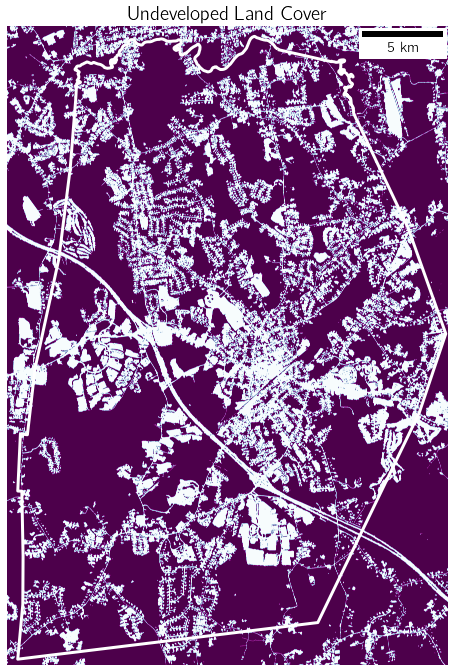
\includegraphics[width=0.5\textwidth]{figures/developed.png}
\caption{Developed land cover is shown in white and undeveloped areas are in dark purple. The town border is also outlined in white. }
\end{wrapfigure}
In recent years, Franklin residents have been concerned with the rate and breadth of development in the community. In the November 2021 election, two incumbent members of the Planning Board (serving for a combined 30 years on the board) lost to two new candidates. Newly elected Beth Wierling and Jennifer Williams share similar philosophies on development. In an interview prior to the election, Williams stated, "I believe we should be more thoughtful about where and how we clear land, even when subdivisions and new homes fall within approved current regulations and by-laws" (Jennifer Williams, 2021). It is believed that this concern was a contributing factor in the community's support of CPA adoption in 2020, since in 2007 the community voted against adopting the CPA (CPC Report). Although there are highly developed areas, there are also relatively undeveloped areas (Figure 2). 
The town government has compiled several goals both in a 2013 Master Plan and in a 2020 Open Space and Recreation Plan, and below are several relevant goals (Franklin Planning and Community Development, 2020 and 2016 Open Space and Recreation Plan). 
\begin{itemize}
\setlength\itemsep{0.0em}
    \item "Preserve and enhance existing unprotected natural and open space resources in Franklin"
    \item "Protect, preserve and enhance Franklin’s natural resources"
    \item "Implement growth management, sustainable development and low impact development techniques to preserve, protect and enhance the town's natural, cultural and historic resources"
     \item "Maximize recreational opportunities to meet the community’s evolving needs by maintaining current inventory of facilities and programs and by providing new facilities and programs for both active and passive recreation"
    \item  "Protect natural, historical and cultural resources and maintain Franklin's New England character"
    \item "Preserve and protect the Town’s Water Resources"
    \item Sources: Franklin Planning and Community Development, 2020 and 2016 Open Space and Recreation Plan
\end{itemize}  
Franklin is still in the beginning stages of creating a strategy for use of CPA funds. The following report details several strategies for land acquisition with a focus on the creation of new protected open spaces. 


%------------------------------------------------------------------------------------------%
\section{Methods}  
All data sets used are publicly available. First, parcels were identified along with their assessed value as of 2020. Parcels which are already protected, parcels assessed under Chapter 61, and parcels already owned by the Town of Franklin were excluded from the analysis (Figure 3). Protected areas fall into four categories based on the time frame of protection. The categories are in perpetuity, temporary, limited, or none. Table 1 shows some areas in Franklin that are protected under each category. The "none" category includes land that is not legally protected but includes scout camps, private golf courses, and private woodlands.

Four land cover types are considered. Prioritization of each land cover advances the town's goals of preserving, protecting, and enhancing natural areas.
\begin{enumerate}
\setlength\itemsep{0.0em}
    \item Priority habitat of rare species
    \item Forest
    \item Wetland
    \item Undeveloped Land
\end{enumerate}  
Priority habitat areas, forest cover, wetland area, and undeveloped areas were each considered as a target land cover (Table 2). Focus on each of these land covers helps to advance the town's goals listed in the Master Plan and Open Space Plan. In each set of analyses, one land cover is selected for focus, and three forms of maximization were used separately for each variable. 
\begin{enumerate}
\setlength\itemsep{0.0em}
    \item Optimal allocation
    \item Largest parcels
    \item Least expensive parcels
\end{enumerate}  

\begin{table}[htbp]
  \centering
  \caption{Types of land protection and sample of land protected in Franklin, MA. Most land is categorized as protected in perpetuity. This is land that is legally protected and often owned by the municipality or state. Land protected in a limited status is legally protected, but not in perpetuity.}
  \resizebox{\textwidth}{!}{
   \begin{tabular}{@{}llr@{}} 
        \toprule
        \multicolumn{1}{c}{Protection Type} & \multicolumn{1}{c}{Sample in Franklin, MA}                                       & \multicolumn{1}{c}{Total Area (acres)} \\ \midrule
        In Perpetuity                       & Franklin State Forest, Charles River Natural Valley Storage Area, Well \#5 & 3925.5                                 \\
        Temporary                           & None                                                                       & 0.0                                    \\
        Limited                             & JFK Elementary School, King Street Park, St. Mary's Cemetery               & 292.1                                  \\
        None                                & Franklin Country Club, Maplegate Country Club                              & 158.3                                  \\ \bottomrule
        \end{tabular}
        }
\end{table}



All parcels with any priority habitat areas were included for analysis. For forest and wetland land cover, each parcel must contain at least one acre of the selected cover. This is an arbitrary cutoff, but it helps prevent the selection of separate parcels that are small and do not help advance the goal of land protection. To be considered an undeveloped parcel, the parcels must include greater than one acre of undeveloped land and is less than 50\% developed land. This is again an arbitrary cutoff. 

In the optimal allocation method, each qualifying parcel has a calculated cost per land cover where the assessed value is divided by the target land area. Please refer to the appendix for a map of land value per area. The parcels are then sorted in ascending order based on the cost per land cover. Parcels are selected until the budget is exhausted. This is called the optimal method because the parcels are selected based on their cost per area, so the result is the largest area for the best value within the budget. When selecting for largest parcels, qualifying parcels are sorted from largest to smallest. Parcels are also selected in order until the budget is exhausted. For the least expensive parcel selection method, the qualifying parcels are sorted based on assessed value in ascending order and selected in order until the budget is exhausted. 
\begin{table}[htbp]
\centering
\caption{Selected variables. Below is a table of data sets that were used in the analysis. Each includes the link to the source, except for Tax Parcel CSV which was provided by personal communication from Franklin's Director of Assessing (November, 2021)}
\begin{tabular}{@{}ll@{}}
\toprule
\multicolumn{1}{c}{Data Type} & \multicolumn{1}{c}{Purpose}             \\ \midrule
\href{https://www.mass.gov/info-details/massgis-data-municipalities}{Town Boundary}                                               & Clip data to relevant spatial extent              \\
\href{https://www.mass.gov/info-details/massgis-data-property-tax-parcels}{Tax Parcels}                                           & Provide spatial boundaries for each parcel        \\
\href{https://www.fisheries.noaa.gov/inport/item/54917}{Land Cover 2016}                                                          & Categorize and calculate land cover of parcels \\
\href{https://www.mass.gov/info-details/massgis-data-protected-and-recreational-openspace}{Protected and Recreational Open Space} & Identification of existing protected areas        \\
\href{https://www.mass.gov/info-details/massgis-data-nhesp-priority-habitats-of-rare-species}{Priority Habitat of Rare Species}   & Identification of parcels with priority habitats  \\
Tax Parcel CSV                                                                                                                    & Obtain assessed value of each parcel              \\ \bottomrule
\end{tabular}
\end{table}


The budget used for this analysis is \$1,000,000. The estimated annual CPA revenue is approximately \$1,000,000 and 10\% must be allocated for open space (Community Preservation Act Fact Sheet). The \$1,000,000 selected budget represents approximately ten years worth of CPA revenue allocated for open space. 

\begin{table}[htbp]
\centering
  \caption{Types of land protection and examples in Franklin, MA. Most land is categorized as protected in perpetuity. This is land that is legally protected and often owned by the municipality or state. Land protected in a limited status is legally protected, but not in perpetuity.}
   \resizebox{0.95\textwidth}{!}{
\begin{tabular}{cccr}
\hline
\multicolumn{1}{c}{Category} & Target Land Use           & Tax Assessment                                      & \multicolumn{1}{c}{Franklin Acres} \\ \hline
61                           & Forestry                  & Based on market value of potential forest products &   0                                 \\
61 A                         & Agriculture               & Based on market value of potential farm products   &   522.9                             \\
61 B                         & Open Space and Recreation & 75\% reduction in assessed value                   &   650.6                             \\ \hline
\end{tabular}}
\end{table}
In Massachusetts, Chapter 61 is a program that provides tax breaks to enrolled land owners. Most properties are assessed based on the value at their "highest and best use,” or the value that the land would have if it was developed, but land enrolled in a Chapter 61 program is assessed differently. There are three categories of Chapter 61 programs (Table 3). For the following analyses, lands assessed under Chapter 61 regulations have been excluded, although they are a valuable town resource (Figure 3). They have been excluded because of the different assessment scheme, and in this analysis, assessed value is used as the measure of land value and cost. When including these parcels, they are often selected due to their low assessed value. Their exclusion in the analysis does not indicate a lack of importance. These parcels are larger than five acres and largely undeveloped, so they offer valuable natural services. They have been excluded due to the decreased assessed value and these areas are likely not at risk for development. Since landowners must enroll and renew participation annually, these landowners have an incentive to maintain their land as undeveloped (Van Fleet et al.). Municipalities have the right of first refusal when Chapter 61 properties are being sold. If these parcels do come up for sale, the town should consider acquisition. Figure 3 shows the areas that have been excluded based on their protected status. 
\begin{figure}[hbtp]
    \centering
    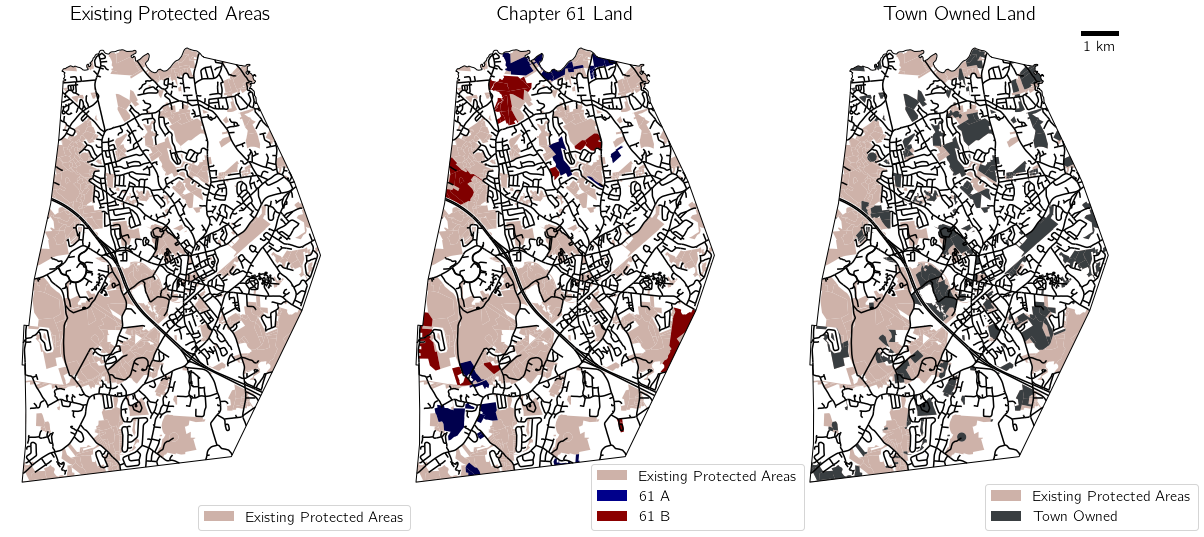
\includegraphics[width = 0.8\textwidth]{figures/existing_prot.png}
    \caption{Existing protected areas. On the left, all lightly shaded areas are excluded from the analysis and are listed as protected based on the MassGIS Protected and Recreational OpenSpace shapefile. In the middle, protected areas are shaded and areas assessed based on the Chapter 61 program are color coded. On the right, town owned land is shaded. Many town owned parcels overlap with the protected areas.}
\end{figure}
\section{Results}
\subsection{Priority Habitat} 
The total area of priority habitat in the municipality is small compared to forest or wetland areas, so there are fewer parcels for selection. Table 4 shows the species that are of priority which are found in Franklin, MA. 
\begin{table}[h]
\caption{Rare species found in Franklin, MA sorted by most recent observation (\href{https://www.mass.gov/info-details/rare-species-viewer}{Rare species viewer})}
\resizebox{\textwidth}{!}{%
\begin{tabular}{@{}lllll@{}}
\toprule
\multicolumn{1}{c}{\textbf{Common Name}} & \multicolumn{1}{c}{\textbf{Scientific Name}} & \multicolumn{1}{c}{\textbf{Taxonomic Group}} & \multicolumn{1}{c}{\textbf{MESA Status}} & \multicolumn{1}{c}{\textbf{Most Recent Obs.}} \\ \midrule
Wood Turtle                              & Glyptemys insculpta                          & Reptile                                      & Special Concern                          & 2016                                          \\
Eastern Box Turtle                       & Terrapene carolina                           & Reptile                                      & Special Concern                          & 2015                                          \\
Least Bittern                            & Ixobrychus exilis                            & Bird                                         & Endangered                               & 1992                                          \\
Small-flowered Buttercup                 & Ranunculus micranthus                        & Vascular Plant                               & Endangered                               & 1910                                          \\
Stiff Yellow Flax                        & Linum medium var. texanum                    & Vascular Plant                               & Threatened                               & 1886                                         \\ \bottomrule          
\end{tabular}}
\end{table}
Priority habitats are limited to the north west corner of Franklin, near Plain St., and the eastern town border. In the three selection methods, optimal, largest, and least, parcels from both areas are selected each time (Figure 4). 

In the optimal selection method there are eight parcels selected which total about 38 acres total, 84\% of which is priority habitat, and 75\% of the selected land area borders a parcel that is already protected (Table 5). This method does not protect the most land area of the three methods, but since it it the "optimal allocation" this method protects the most land area at the lowest cost per area. 

When the largest parcels that contain priority habitat are selected, there are three parcels which cover ten acres of land, 90\% of which is an area of priority habitat. Visually this method seems similar to the optimal selection method, but this method selects eight fewer acres of property. Interestingly, this is the most efficient method of selection where 90\% of the selected land area is priority habitat

The least expensive method selects 12 parcels that add to 49 acres, but only 46\% of those acres are areas of priority habitat. Although the largest area of land is selected in the least expensive method, it is the least efficient. In all three selection methods, between 75\% and 76\% of the parcel land area border an already protected area. 
\begin{figure}[hbtp]
    \centering
    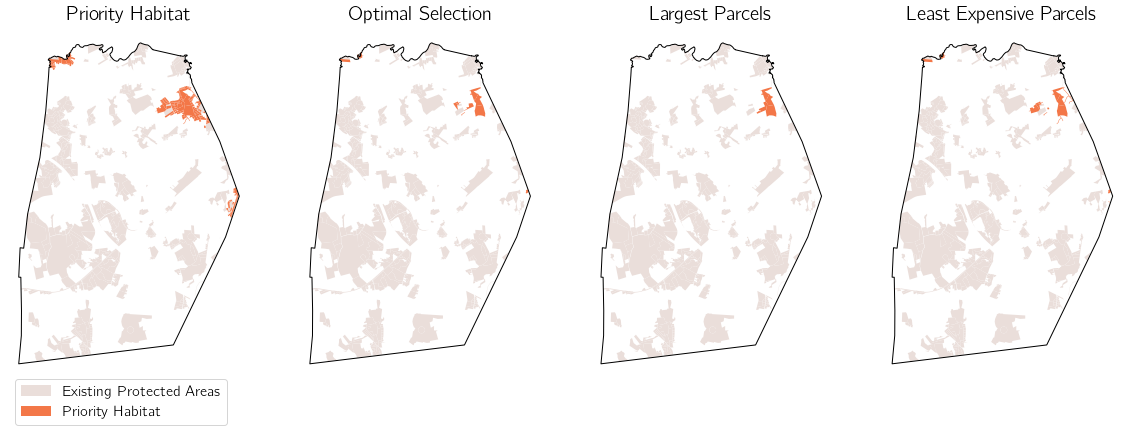
\includegraphics[width = \textwidth]{figures/n_61prihab.png}
    \caption{Selected parcels of priority habitat excluding existing protected land using three optimization methods. }
\end{figure}
\begin{table}[hbtp]
\caption{Summary of priority habitat parcel selections using three methods.}
  \resizebox{\textwidth}{!}{
\begin{tabular}{@{}crrrrrr@{}}
\toprule
 & \multicolumn{1}{c}{\begin{tabular}[c]{@{}c@{}}Number of\\ Selected Parcels\end{tabular}} & \multicolumn{1}{c}{\begin{tabular}[c]{@{}c@{}}Area \\ (acres)\end{tabular}} & \multicolumn{1}{c}{\begin{tabular}[c]{@{}c@{}}Area of Priority Habitat\\ (acres)\end{tabular}} & \multicolumn{1}{c}{Efficiency \%} & \multicolumn{1}{c}{Budget Used} & \multicolumn{1}{c}{\begin{tabular}[c]{@{}c@{}}\% Area Borders\\ Protected Land\end{tabular}} \\ \midrule
Optimal & 8 & 38 & 32 & 84 & 935000 & 75 \\
Largest & 3 & 30 & 27 & 90 & 839200 & 75 \\
Least Expensive & 12 & 49 & 23 & 46 & 976100 & 76 \\ \bottomrule
\end{tabular}}
\end{table}
\subsection{Forest}
 There are forested areas throughout Franklin, but the most forested areas are south of Route 495 which can be seen cutting through Franklin in a north-west to south-east line (Figure 5). Areas such as the Franklin State Forest or Southern New England Trunkline Trail are already protected.
 
 In the optimal selection process, 18 parcels with forests were selected which cover a total of 180 acres, and 113 are categorized as forest cover. This method selects the most land area of the three forest selection methods (Table 6). When examining the optimally selected parcels, 78\% of the land is part of a parcel that borders an already protected parcel. Although the 18 parcels are relatively small, most border an area that is already protected. 
 
 In the largest parcel selection method, one parcel that is nearly 47 acres large and assessed at \$818,400 is selected. This parcel is on Upper Union St. and is owned by the Cistercian Nuns. This parcel borders an existing protected area and is 75\% forested. According to their website, the Order of Cistercians of the Strict Observance requires, "The sisters are to be concerned about conservation of the environment and to manage natural resources prudently" (Care for Creation). In total, the Cistercian Nuns own 511 acres of land in Franklin. 
 
 In contrast with the one parcel selected in the largest selection method, the least expensive method selects 40 parcels. For example, two parcels are owned by condominium complexes and two are owned by electric and oil companies.These selected parcels are largely separate from each other and separate from existing protected areas, since 29\% of the selected parcel areas border an existing protected area. The selected parcels cover an area of 101 acres of which 73 acres are forested.  
 
\begin{figure}[hbtp]
    \centering
    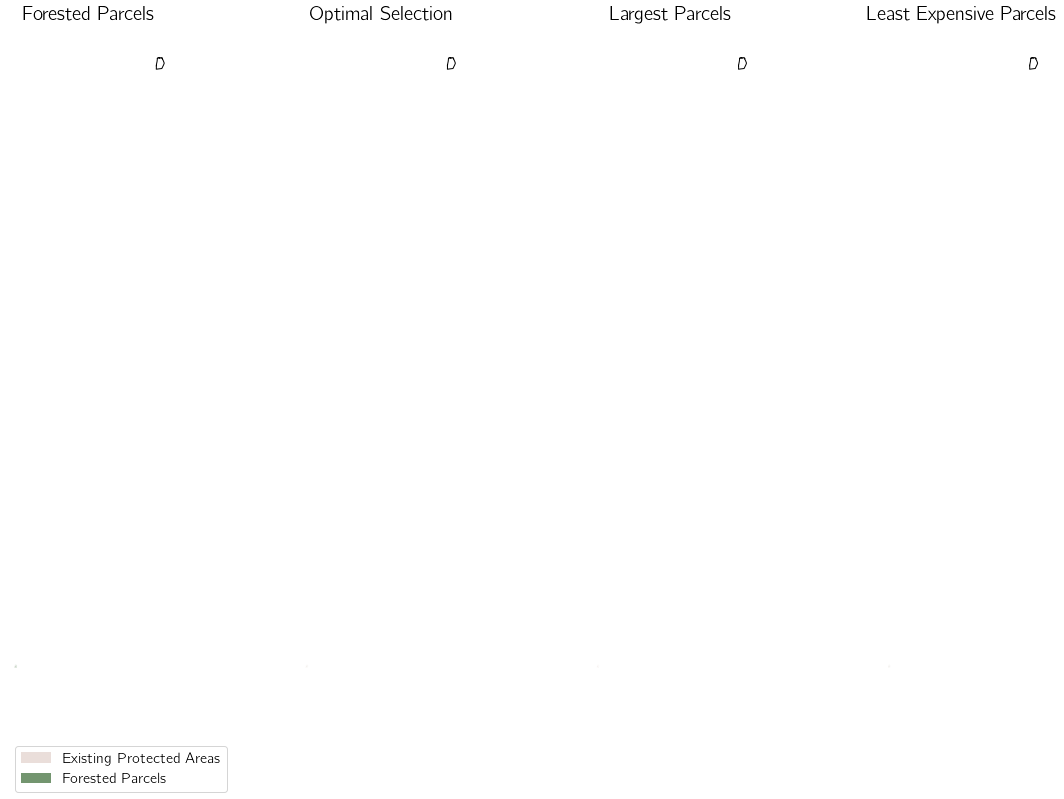
\includegraphics[width = \textwidth]{figures/n_61forest.png}
    \caption{Selected parcels of forest excluding existing protected land using three optimization methods. }
\end{figure}

\begin{table}[hbtp]
\caption{Summary of forested parcel selections using three methods.} 
  \resizebox{\textwidth}{!}{
\begin{tabular}{@{}crrrrrr@{}}
\toprule
 & \multicolumn{1}{c}{\begin{tabular}[c]{@{}c@{}}Number of\\ Selected Parcels\end{tabular}} & \multicolumn{1}{c}{\begin{tabular}[c]{@{}c@{}}Area \\ (acres)\end{tabular}} & \multicolumn{1}{c}{\begin{tabular}[c]{@{}c@{}}Area of Forest\\ (acres)\end{tabular}} & \multicolumn{1}{c}{Efficiency\%} & \multicolumn{1}{c}{Budget Used} & \multicolumn{1}{c}{\begin{tabular}[c]{@{}c@{}}\% Area Borders\\ Protected Land\end{tabular}} \\ \midrule
Optimal & 18 & 180 & 113 & 63 & 951200 & 78 \\
Largest & 1 & 47 & 35 & 75 & 818400 & 100 \\
Least Expensive & 40 & 101 & 73 & 73 & 964400 & 29 \\ \bottomrule
\end{tabular}}
\end{table}
\subsection{Wetland}
Much of the connected wetlands in Franklin are owned by the town or protected by another source. For example, the Army Corps of Engineers own land along Mine Brook which runs across the town from south east to north west. Despite this, there are significant areas of unprotected wetlands (Figure 6).  

Using the optimal selection approach, eighteen parcels were selected, and include areas along Lincoln Street, Pond Street, and Chestnut Street. Of the 162 selected acres, 90 of these acres are categorized as wetlands, and 78\% of the area borders a protected parcel. 

The largest parcel selection method selects three parcels throughout the municipality. Of the 89 acres covered by this selection, 44 acres are wetland. This has the 49\% efficiency which is the lowest of all methods and land uses (Table 7). These three parcels each border an area that is already protected. Two of the selected parcels are also selected in the optimal allocation method. 

Similarly to the previous land covers, the least expensive method selects the largest number of parcels. In this method 24 parcels that cover 111 acres are selected, and 66 acres of the selected parcels are wetlands. These parcels are smaller than those selected in the optimal selection method or the largest parcel selection method, and 42\% of the area borders a protected parcel. 
 
\begin{figure}[hbtp]
    \centering
    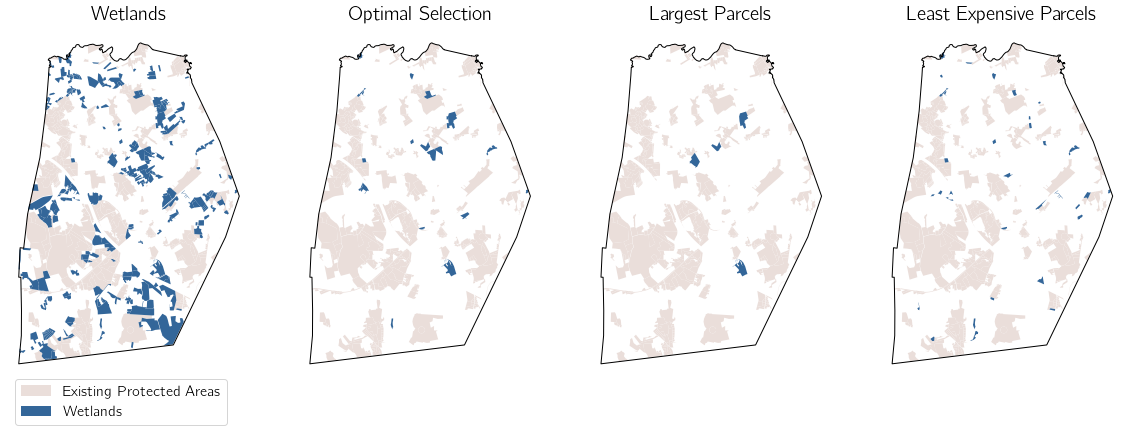
\includegraphics[width = \textwidth]{figures/n_61wetland.png}
    \caption{Selected parcels of wetlands excluding existing protected land using three optimization methods.}
\end{figure}
\begin{table}[hbtp]
\caption{Summary of selected wetland parcels. } 
  \resizebox{\textwidth}{!}{
\begin{tabular}{@{}crrrrrr@{}}
\toprule
 & \multicolumn{1}{c}{\begin{tabular}[c]{@{}c@{}}Number of\\ Selected Parcels\end{tabular}} & \multicolumn{1}{c}{\begin{tabular}[c]{@{}c@{}}Area \\ (acres)\end{tabular}} & \multicolumn{1}{c}{\begin{tabular}[c]{@{}c@{}}Area of Wetlands\\ (acres)\end{tabular}} & \multicolumn{1}{c}{Efficiency\%} & \multicolumn{1}{c}{Budget Used} & \multicolumn{1}{c}{\begin{tabular}[c]{@{}c@{}}\% Area Borders\\ Protected Land\end{tabular}} \\ \midrule
Optimal & 18 & 180 & 113 & 63 & 951200 & 78 \\
Largest & 3 & 89 & 44 & 49 & 864500 & 100 \\
Least Expensive & 24 & 111 & 66 & 60 & 961800 & 42 \\ \bottomrule
\end{tabular}}
\end{table}
\subsection{Undeveloped Land}
Undeveloped land is the least restrictive land use category used. Undeveloped land excludes area categorized as impervious or developed open space and includes forest, and wetlands, as well as cultivated land, pasture, or shrub/scrub. These areas can be found throughout the municipality (Figure 7). Because of this expansive definition, this land cover allows for the selection of the most land area. 

The optimal selection method selects 202 acres of land 87\% of which is undeveloped, and 91\% of the land area borders an existing protected area (Table 8). Two of these parcels are owned by condominium complexes, and one selected parcel is owned by the Cistercian Nuns who, in addition to the forested parcel which was selected in the forest largest parcel selection method, have pasture with sheep and a solar farm. It seems that forested parcels in south eastern Franklin are large, but do not offer the best price per area.  

When using the largest parcel selection method, three parcels are selected which total 89 acres and 75 acres are undeveloped. All of the selected parcels border an already protected area. 


 The least expensive method selects 54 parcels, which is the most of any selection method, but these parcels sum to nearly 89 acres, and 86 acres are undeveloped. These parcels are disjointed and only 32\% of the land borders a parcel that is already protected. 
\begin{figure}[hbtp]
    \centering
    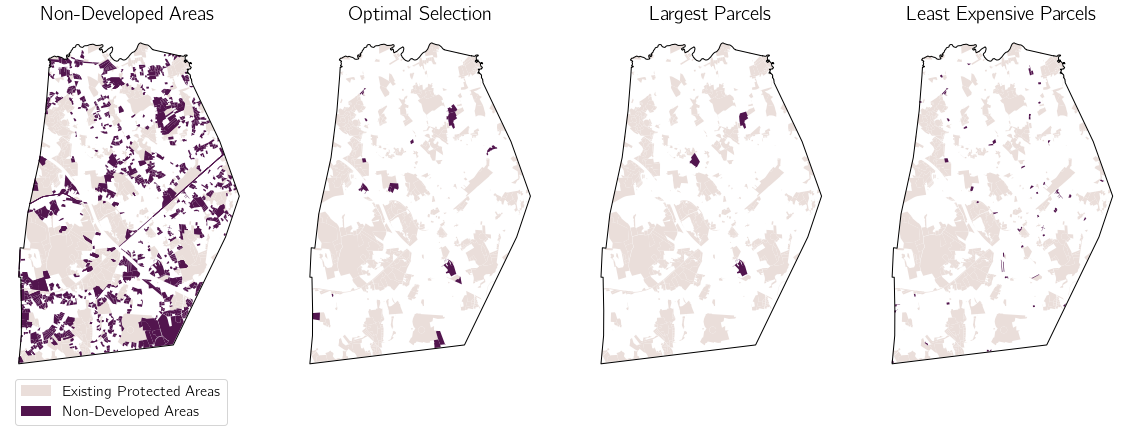
\includegraphics[width = \textwidth]{figures/n_61ndev.png}
    \caption{Selected parcels of undeveloped land excluding existing protected land using three optimization methods. }
\end{figure}

\begin{table}[hbtp]
\caption{Summary of selected undeveloped parcels.} 
  \resizebox{\textwidth}{!}{
\begin{tabular}{@{}crrrrrr@{}}
\toprule
 & \multicolumn{1}{c}{\begin{tabular}[c]{@{}c@{}}Number of\\ Selected Parcels\end{tabular}} & \multicolumn{1}{c}{\begin{tabular}[c]{@{}c@{}}Area \\ (acres)\end{tabular}} & \multicolumn{1}{c}{\begin{tabular}[c]{@{}c@{}}Area of Undeveloped\\ (acres)\end{tabular}} & \multicolumn{1}{c}{Efficiency\%} & \multicolumn{1}{c}{Budget Used} & \multicolumn{1}{c}{\begin{tabular}[c]{@{}c@{}}\% Area Borders\\ Protected Land\end{tabular}} \\ \midrule
Optimal & 18 & 202 & 176 & 87 & 995000 & 91 \\
Largest & 3 & 89 & 75 & 84 & 864500 & 100 \\
Least Expensive & 54 & 89 & 86 & 97 & 971300 & 32 \\ \bottomrule
\end{tabular}}
\end{table}
\subsection{Summary}
\begin{figure}[hbtp]
    \centering
    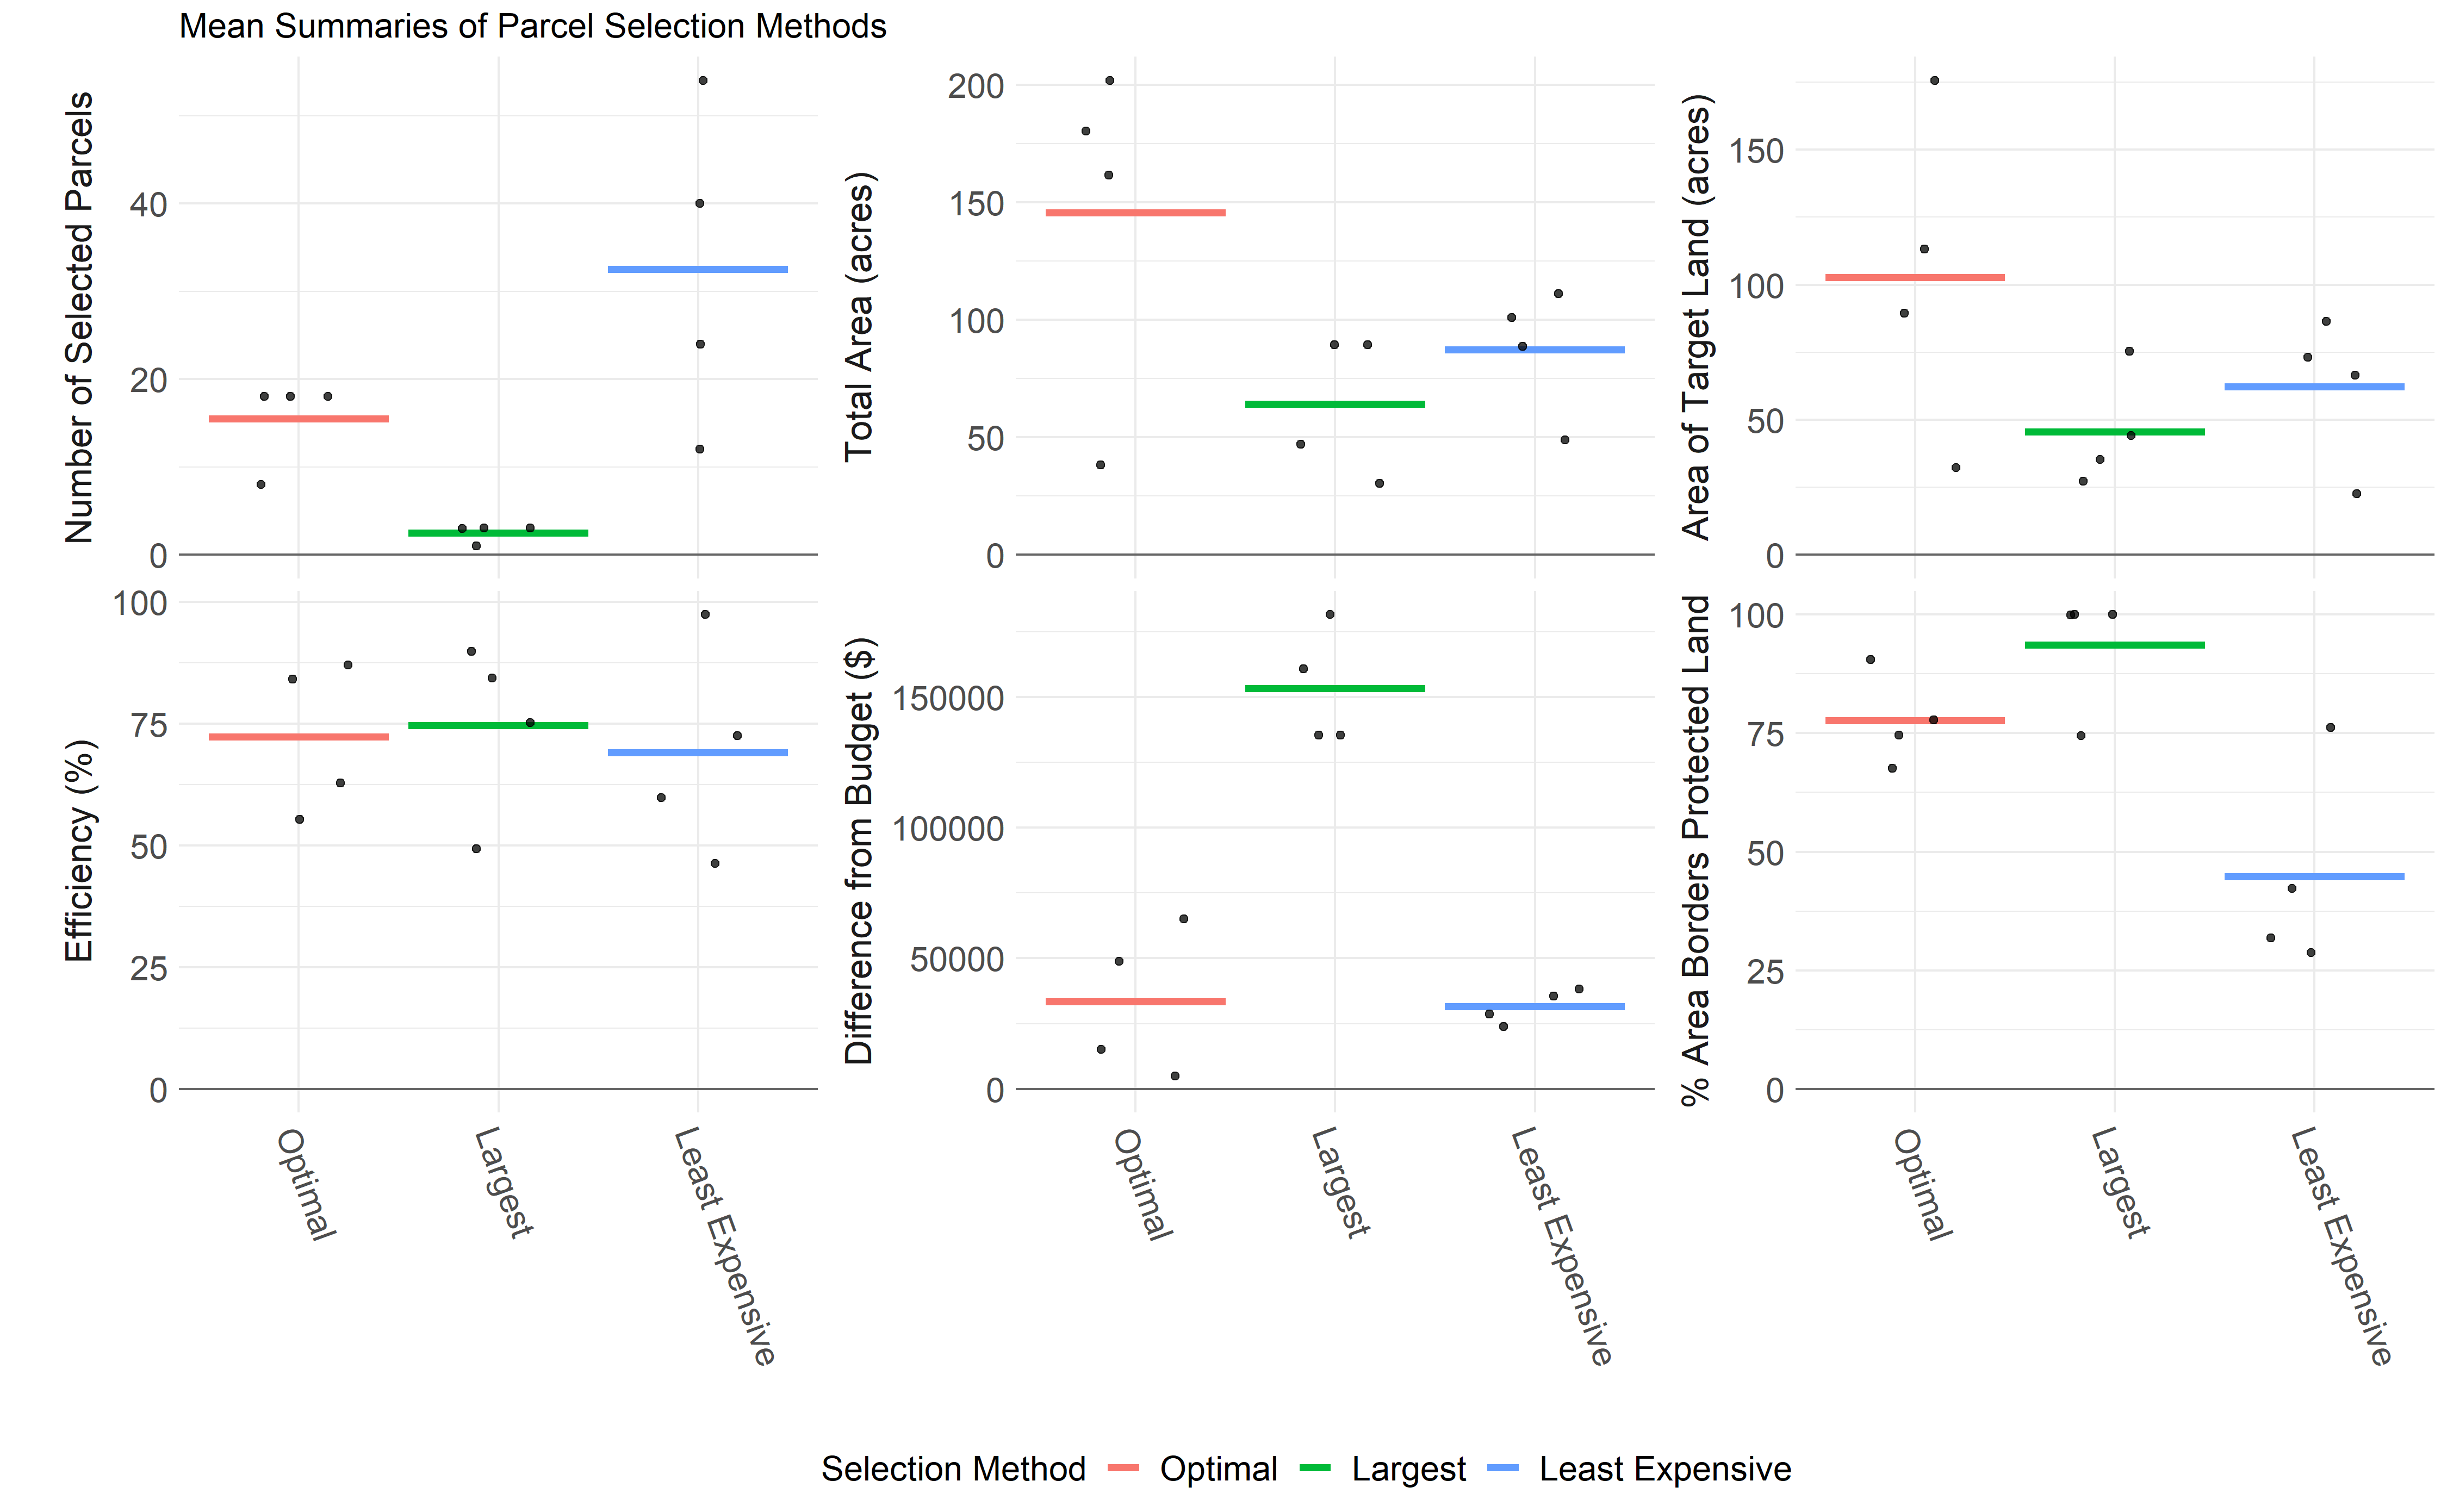
\includegraphics[width = \textwidth]{figures/summary.png}
    \caption{Means of selected measures for each parcel selection method. The colored line shows the mean for the selection method, and the points show the values of each of the four land covers, priority habitat, forest, wetlands, and undeveloped land. }
\end{figure}
Figure 8 shows summaries for each value used to evaluate the parcel selection methods. The colored line shows the mean for the selection method, and the points show the values calculated for each of the four land covers. The three selection methods have, on average, similar efficiency rates that are around 72\%. 

The optimal selection method selects the  most area (acres) and the most area of the target land cover (acres), although it does not select the greatest number of parcels. With this method, approximately 75\% of the selected land area borders a parcel that is already protected, which is between the average of the largest method and the least expensive method. 

The largest parcel selection method selects the least number of parcels, the least total area, and the least area of target land cover. This selection method also has the largest difference from the budget, which means that the most money is left unused. The largest parcel selection method selects the highest proportion of land area that borders an existing protected parcel. This is likely due to the small number of parcels selected. If only one parcel is selected, and that parcel borders protected areas, the proportion of land area that borders an existing protected parcel is one.

The least expensive method selects the most parcels, on average, which makes logical sense. When there are smaller, less expensive parcels, more can be selected within the budget. Although the largest number of parcels are selected, the total area selected is less than that of the optimal selection method. The least expensive parcel selection method selects the lowest proportion of land area that also borders a protected parcel at 45\%. The difference from the budget is similar to that of the optimal selection method. 

\begin{figure}[hbtp]
    \centering
    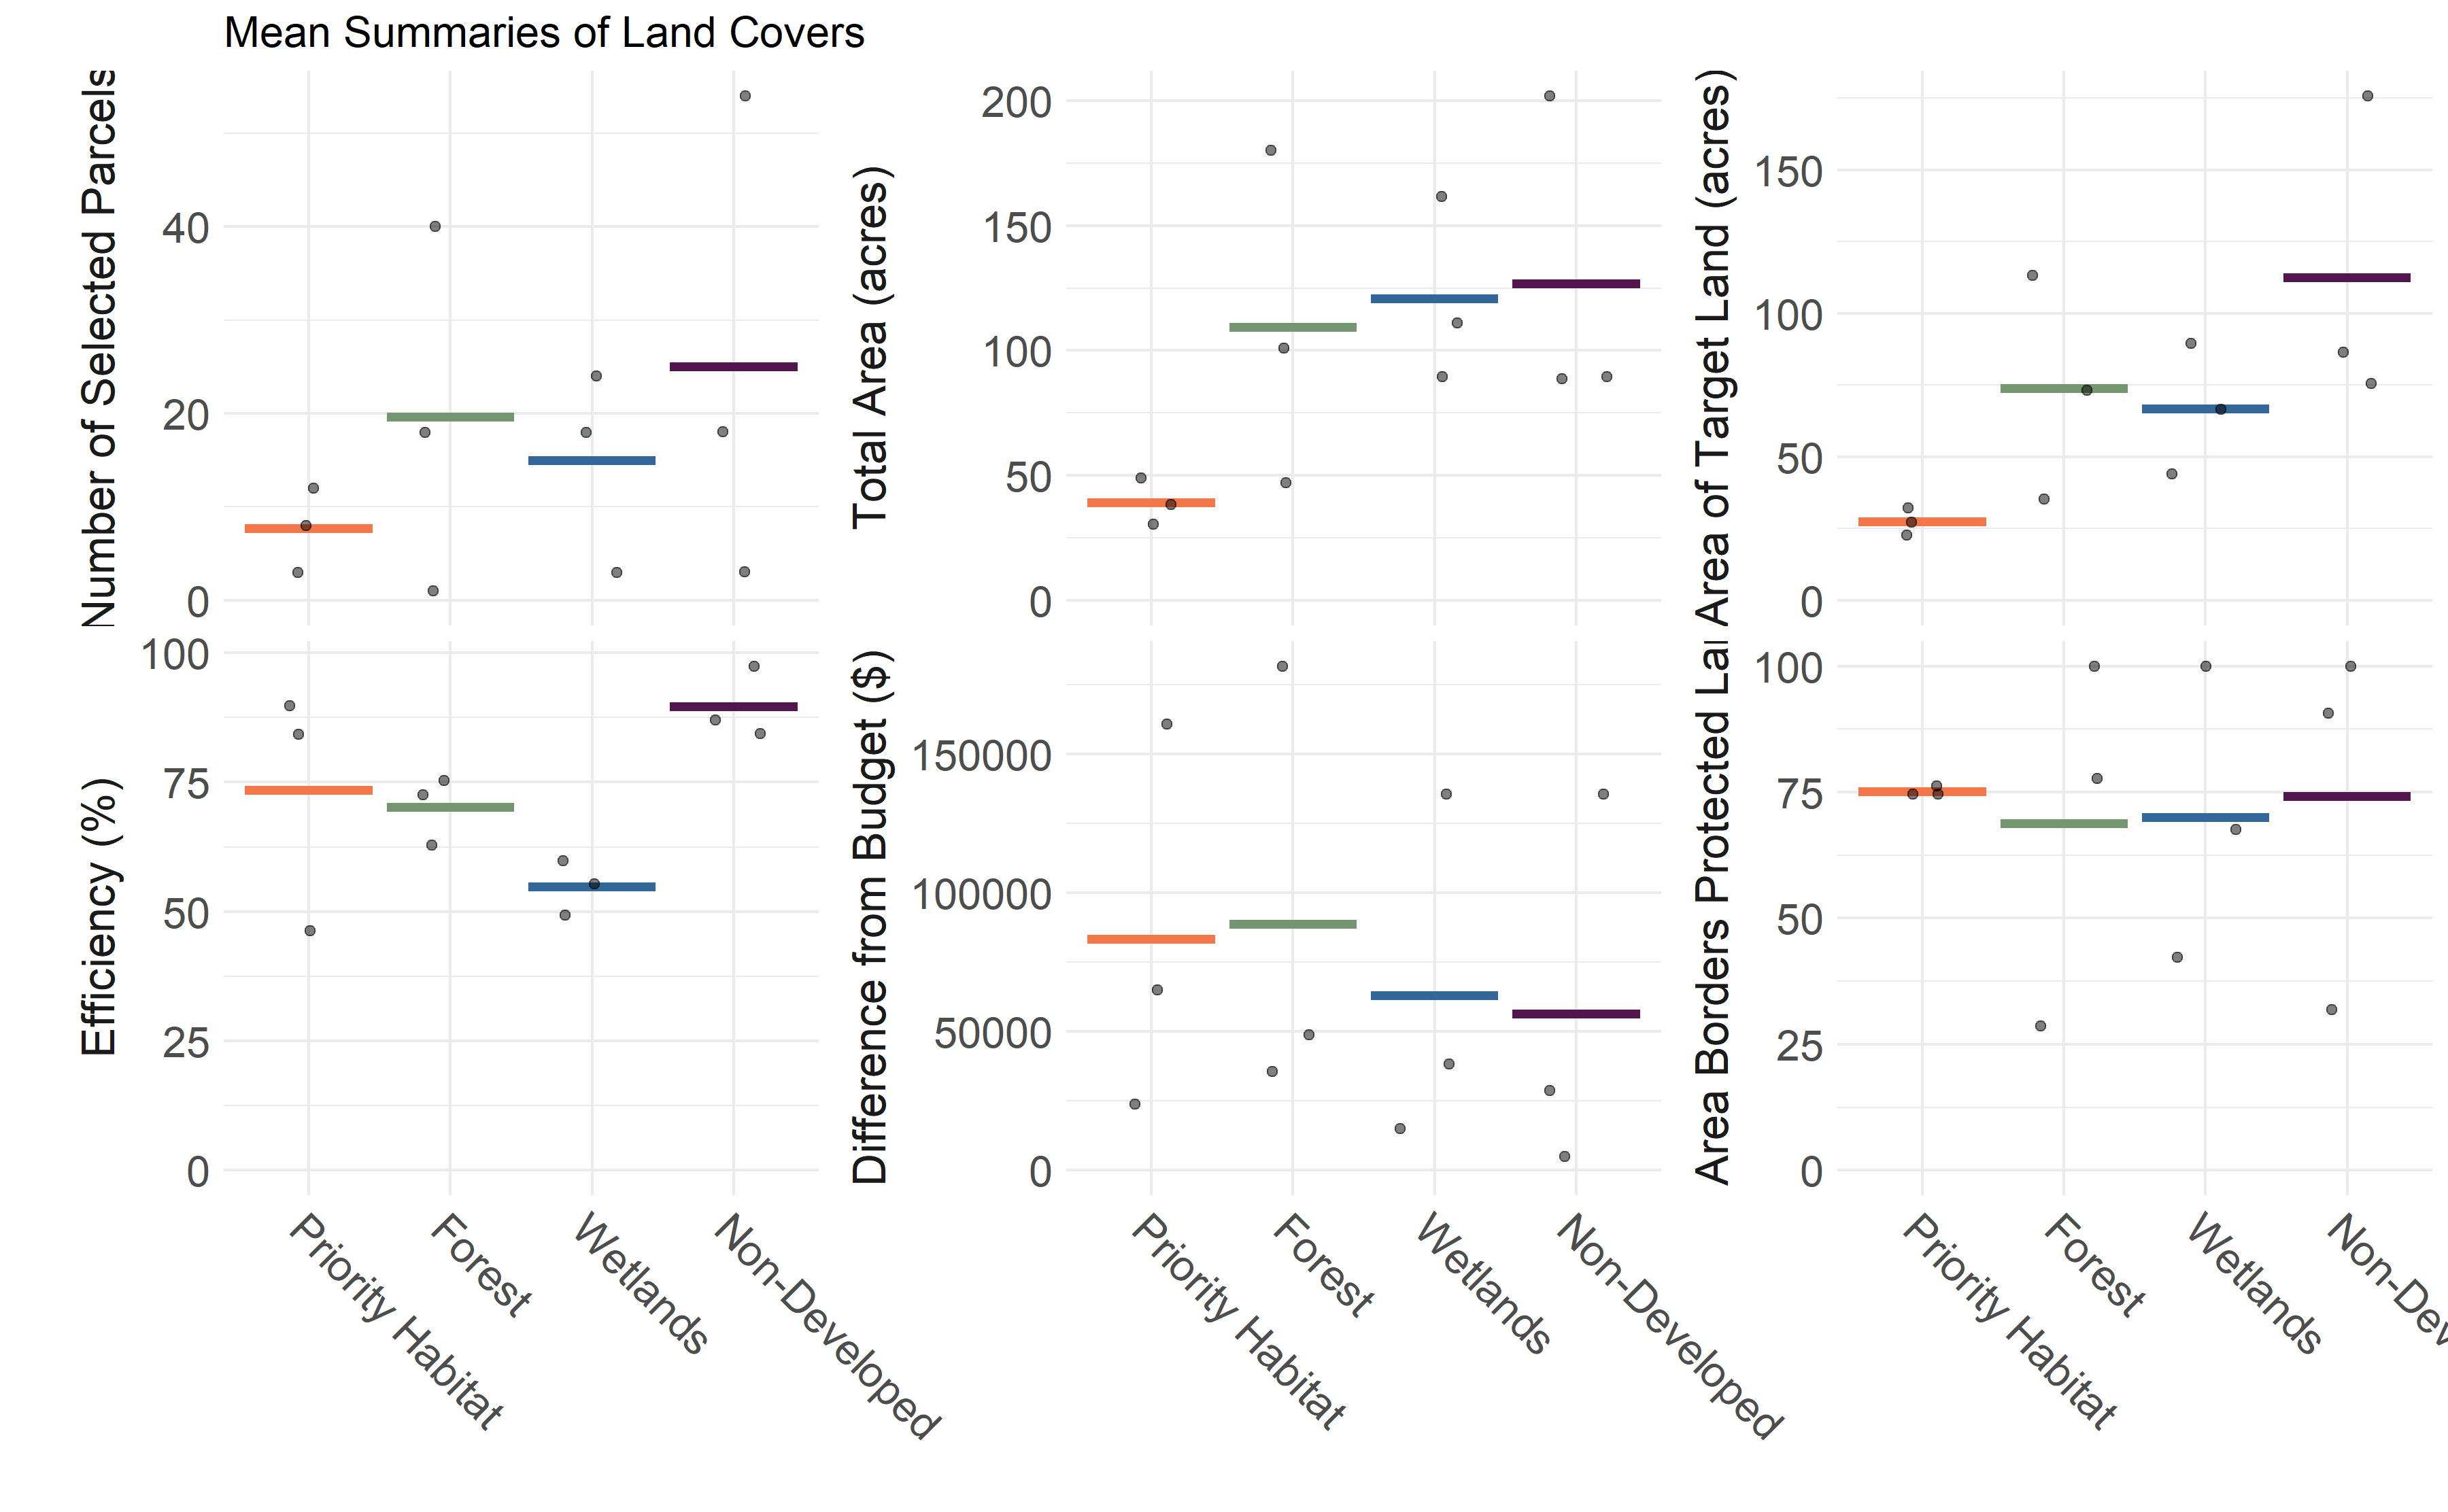
\includegraphics[width = \textwidth]{figures/summary_lc.png}
    \caption{Means of selected measures for each selected land cover. The colored line shows the mean for the land cover, and the points show the values of each of the three selection methods.}
\end{figure}
Figure 9 shows a similar plot, but summarized by the selected land cover. Each bar shows the mean for the land cover and each point shows the values for each of the selection methods. Each of the land cover selections has a similar average percent area bordering an existing protected area.  

The priority habitat land cover has the lowest number of selected parcels and the least area selected. This is likely because there is not much priority habitat in the town, so there are fewer parcels to select. Priority habitat selections have an efficiency of nearly 75\%, and about 75\% of selected land area borders a protected area. 

Forested areas and wetlands have similar moderate results. Forests have a higher number of selected parcels and target land area than wetlands, but there are fewer total acres selected in the forested selections than total acres selected when using wetlands as the target land cover. Forest selections have a moderate efficiency when compared to the other land covers. The difference from the budget is the greatest for forested areas. This average is larger than other land covers, likely due to the single parcel selected in the largest parcel selection method. Wetland area selections have moderate results for most of the plots in Figure 9. Wetlands stands out in efficiency, though, with the lowest average efficiency of the land uses. On average, just over half of the land area of selected parcels is wetland area. 

Non-developed land has the highest average number of selected parcels, area selected, and efficiency. This is probably due to the high occurrence of non-developed parcels, so there are more areas to select. Non-developed land also has the least difference from the budget on average, indicating that the least amount of money would be left unused. 
\section{Discussion}
Each method presented in the above analysis represents a single strategy for conservation. As shown above, each method yields varied results. One assumption of this project is that the data are up to date and accurate. The land cover data (forest, wetlands, developed) were last updated in 2016, so it can be expected that there has been change in land cover since the latest update. Assessed parcel value is used to represent the cost of land acquisition, but it is a simple representation, since there are more elements to acquiring land than simply the assessed value. Additionally, the analysis only considers one land cover at a time. Perhaps the town wants to conserve a variety of land covers rather than exclusively forest, for example. The analysis has used arbitrary cutoffs to determine an "acceptable" parcel for conservation. For example, to be considered in the above analyses, a forest parcel must be at least one acre in area. In reality there could be another cutoff that better suits the needs of the town. Due to these assumptions, the analysis should not be viewed as prescriptive, but rather an evaluation of the town and a set of suggestions.     

On average, the optimal allocation method protects the largest land area and the largest parcel selection method protects the least area. This seems counter-intuitive at first, but when selecting only the largest parcels the budget runs out quickly and fewer areas can be conserved. The least expensive parcel selection method selects the most parcels, on average, but has the fewest borders with existing protected land. The least expensive parcels are often small and separate from each other.  
Overall the optimal allocation method is ideal for parcel selection, since it offers, on average, the most area that is protected within the constraints of a budget. This method though, is an idealization of the world, and this analysis is imperfect by making assumptions to simplify the scope of the project. 

In order to protect the most area, non-developed land should be the target, but the town may have other goals that take into account the quality of the undeveloped land. The optimal parcel selection of non-developed land protects the most area with nearly 90\% of the selected land being undeveloped.  Other factors to consider in future analyses include the benefits of contiguity or the level of threat that a parcel faces. For example, in the least expensive parcel selection method, many parcels are separated from each other, so the town may want to prioritize areas that are adjacent to already protected areas to reduce the edge effect on protected parcels. Additionally, the level of threat that a parcel experiences could be considered. The parcels owned by the Cistercian Nuns are not likely highly threatened, but forested parcels close to recent development projects may be threatened. Forested areas, wetlands, and priority habitat areas each provide value to the town in different ways, and each optimization method presented offers a single option for consideration in systematically conserving land. 

%------------------------------------------------------------------------------------------------------------------------------%
\section{Conclusion}
This project is an exploratory analysis of options for the Town of Franklin's allocation of CPA funds to acquire new open space areas. The optimal allocation method, provides the greatest land area at the best value, and the non-developed land cover is most expansive and covers the most area. If the town's goal is to protect the most area, officials should consider implementing the optimal selection method with non-developed land as the target land area. This is a simplification of reality, since there are a variety of goals that the town is working to achieve. This project provides an outline of potential ways to optimize land acquisition. None is perfect, but each offers insights into a method that the town could consider to more systematically plan land conservation through the use of CPA funds.  
\newline
\newline
All code and files can be found at \url{https://github.com/r-determan/Franklin_OpenSpace}. 
\newpage
\section{Works Cited}
\onehalfspacing
\begin{flushleft}
Care for Creation. Mount Saint Mary’s Abbey. Retrieved January 18, 2022, from \url{https://msmabbey.org/care-for-creation}
\newline
\newline
CPA: An Overview | Community Preservation Coalition. Retrieved December 29, 2021, from \url{https://www.communitypreservation.org/about}  
\newline
\newline
Community Preservation Act Fact Sheet. Retrieved January 17, 2022, from \url{https://www.franklinma.gov/sites/g/files/vyhlif6896/f/uploads/cpa_fact_sheet_3.pdf}
\newline 
\newline
CPC Report | Community Preservation Coalition. Retrieved December 29, 2021, from \url{https://www.communitypreservation.org/cpc-report?report_src=bbzvidkqg|a=dr&rid=241} 
\newline 
\newline
Jennifer Williams. (September 2021). \emph{Franklin Voter Guide.} Retrieved December 29, 2021, from \url{https://www.franklinvoterguide.org/2021-voter-guide/guide-planning-board/jennifer-williams} 
\newline
\newline
MassGIS Data: 2010 U.S. Census | Mass.gov. Retrieved December 19, 2021, from \url{https://www.mass.gov/info-details/massgis-data-2010-us-census}
\newline
\newline
MassGIS Data: Municipalities | Mass.gov.  Retrieved December 1, 2021, from \url{https://www.mass.gov/info-details/massgis-data-municipalities}
\newline
\newline
MassGIS Data: NHESP Priority Habitats of Rare Species | Mass.gov. Retrieved December 10, 2021, from \url{ https://www.mass.gov/info-details/massgis-data-nhesp-priority-habitats-of-rare-species}
\newline
\newline
MassGIS Data: Property Tax Parcels | Mass.gov.Retrieved December 1, 2021, from \url{https://www.mass.gov/info-details/massgis-data-property-tax-parcels}
MassGIS Data: Protected and Recreational OpenSpace | Mass.gov. Retrieved December 10, 2021, from \url{https://www.mass.gov/info-details/massgis-data-protected-and-recreational-openspace}

Office for Coastal Management, 2021: C-CAP Land Cover, Massachusetts, 2016 from 2010-06-15 to 2010-08-15. NOAA National Centers for Environmental Information, \url{https://www.fisheries.noaa.gov/inport/item/54917}. 
\newline
\newline
Rare species viewer | Natural Heritage & Endangered Species Program | Mass.gov. Retrieved January 18, 2022, from \url{https://www.mass.gov/info-details/rare-species-viewer}
\newline
\newline
Taberner, B. W. (2020). \emph{Update on implementation of 2013 master plan}[Memorandum]. Franklin Planning and Community Development. \url{https://www.franklinma.gov/sites/g/files/vyhlif6896/f/uploads/masterplan_update_materials.pdf}  
\newline
\newline
Van Fleet, T., Catanzaro, P., \& Kittredge, D.. \emph{Chapter 61 Programs: Understanding the Massachusetts Ch. 61 Current Use Tax Programs.} \url{https://www.mass.gov/files/documents/2017/10/25/chapter-61-programs.pdf}
\end{flushleft}
\newpage
%------------------------------------------------------------------------------------------------------------------------------%

\section{Appendix}

\begin{figure}[hbtp]
    \centering
    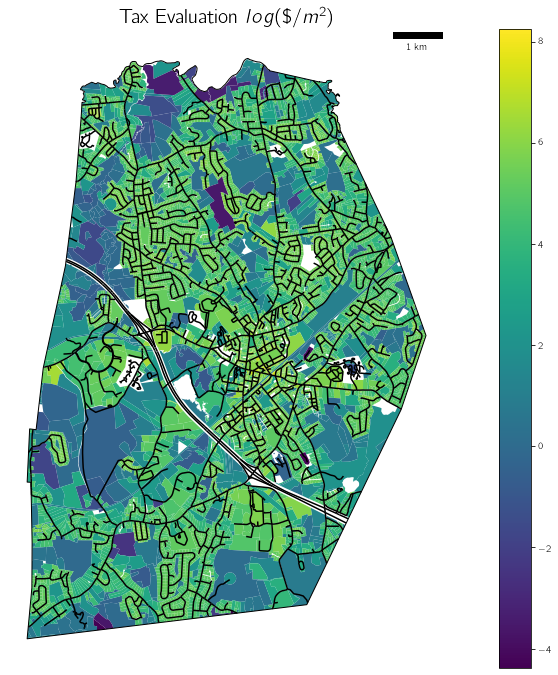
\includegraphics[width=0.75\linewidth]{figures/landval.png}
    \caption{Tax evaluation log(\$/m$^2$). Yellow/green indicates a higher cost per area and blue/purple indicates a lower cost per area. Residential areas have a higher evaluation per m$^2$ when compared to parks or forests. }
\end{figure}

\begin{table}[]
\centering
\caption{Area of selected variables in ascending order. All land includes the selected variables and land not categorized as priority habitat, wetland, developed, or forested. }
\begin{tabular}{@{}lr@{}}
\toprule
\multicolumn{1}{c}{Category} & \multicolumn{1}{c}{Area (acres)} \\ \midrule
Priority Habitat             & 218.5                            \\
Wetland                      & 2276.1                           \\
Developed                    & 3932.1                           \\
Forest                       & 7489.0                           \\
All Land                     & 14381.5                          \\ \bottomrule
\end{tabular}
\end{table}

\begin{figure}[H]
    \centering
    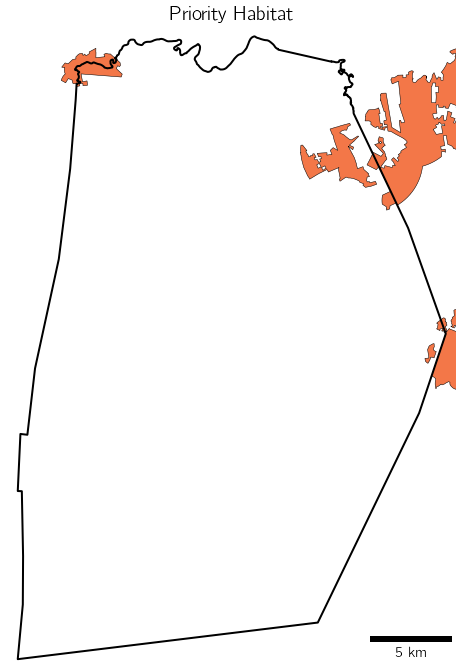
\includegraphics[width=0.75\linewidth]{figures/prihab_cover.png}
    \caption{Priority habitat areas of Franklin, MA.  }
\end{figure}

\begin{figure}[H]
    \centering
    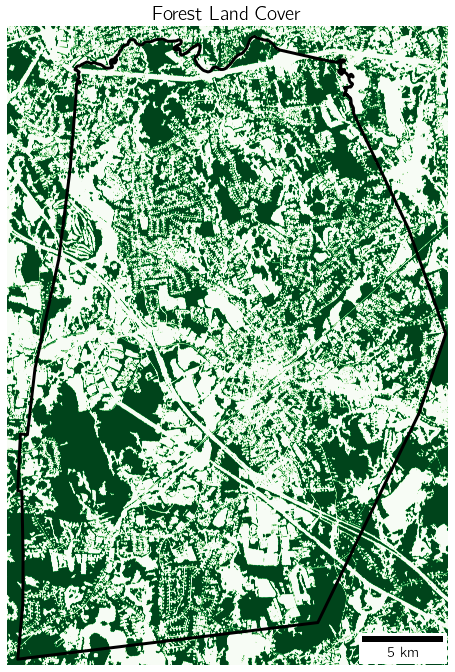
\includegraphics[width=0.75\linewidth]{figures/forest_cover.png}
    \caption{Forest cover of Franklin, MA. Green areas represent deciduous or evergreen forest. One area of note is the protected Franklin State Forest in the south west quadrant of the town. }
\end{figure}

\begin{figure}[H]
    \centering
    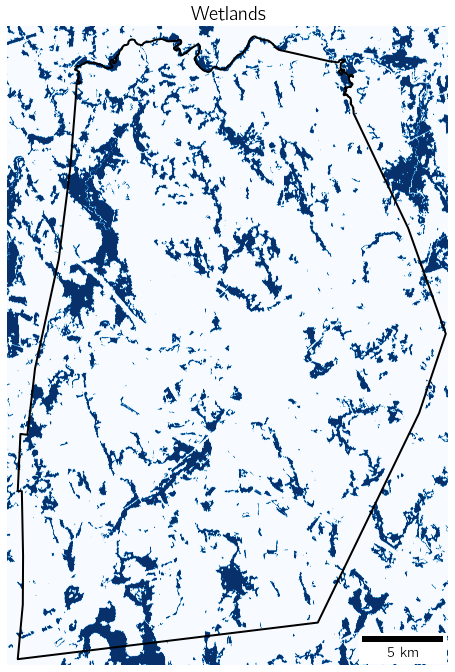
\includegraphics[width=0.75\linewidth]{figures/wet_cover.png}
    \caption{Forest cover of Franklin, MA. Blue areas represent areas categorized as palustrine forested wetland, palustrine scrub/shrub wetland, palustrine emergent wetland. In the north west one can see a large area of connected wetland which is the protected the Army Corps of Engineer's land.  }
\end{figure}


\begin{table}[H]
\resizebox{\textwidth}{!}{%
\begin{tabular}{@{}lrrrrrrr@{}}
\toprule
\multicolumn{1}{c}{Scenario} & \multicolumn{1}{c}{N} & \multicolumn{1}{c}{\begin{tabular}[c]{@{}c@{}}Area \\ (acres)\end{tabular}} & \multicolumn{1}{c}{\begin{tabular}[c]{@{}c@{}}Metric Area \\ (acres)\end{tabular}} & \multicolumn{1}{c}{Efficiency} & \multicolumn{1}{c}{Budget} & \multicolumn{1}{c}{\begin{tabular}[c]{@{}c@{}}Difference \\ from Budget\end{tabular}} & \multicolumn{1}{c}{\begin{tabular}[c]{@{}c@{}}\% Area Borders\\  Protected\end{tabular}} \\ \midrule
Opt. Priority Habitat & 8 & 38 & 32 & 84 & 935000 & 65000 & 75 \\
Largest Priority Habitat & 3 & 30 & 27 & 90 & 839200 & 160800 & 75 \\
Least expensive Priority Habitat & 12 & 49 & 23 & 46 & 976100 & 23900 & 76 \\
Opt. Forest & 18 & 180 & 113 & 63 & 951200 & 48800 & 78 \\
Largest Forest & 1 & 47 & 35 & 75 & 818400 & 181600 & 100 \\
Least expensive Forest & 40 & 101 & 73 & 73 & 964400 & 35600 & 29 \\
Opt. Wetlands & 18 & 162 & 90 & 55 & 984900 & 15100 & 68 \\
Largest Wetlands & 3 & 89 & 44 & 49 & 864500 & 135500 & 100 \\
Least expensive Wet & 24 & 111 & 66 & 60 & 961800 & 38200 & 42 \\
Opt. Non-Dev & 18 & 202 & 176 & 87 & 995000 & 5000 & 91 \\
Largest Non-Dev & 3 & 89 & 75 & 84 & 864500 & 135500 & 100 \\
Least expensive Non-Dev & 54 & 89 & 86 & 97 & 971300 & 28700 & 32 \\ \bottomrule
\end{tabular}}
\end{table}


\end{document}